\subsection{Validation} \label{compvis_anfisvalid}

It has been asserted a number of times in this report (Section \ref{fusion_bounds}, XX) that a physics-informed ANFIS fusion network is expected outperform a standard Naive Bayes (NB) fusion model. It is therefore important to validate this hypothesis with a crude simulation of environmental conditions, and the resulting sensor data to demonstrate how integrating domain knowledge can improve data fusion performance.

\paragraph{Synthetic Data Generation}  

    The reason that ANFIS is expected to work better than NB, is that the assumptions of conditional independance on which NB is based, fail in real world conditions, where there is coupling between the two sensors through the causal physics of the environment. To highlight the shortcomings of NB, we must include this conditional dependence in the model. Here it is chosen to use the \textbf{soil moisture} as a means to do this. It was shown in Section \ref{anfis_rules} that an increase in soil moisture tends to boost the thermal sensor detectability (through increasing the thermal conductivity, which, as shown in Section \ref{conductivity}, increases the thermal return) and to inhibit the radar return (by increasing the electrical conductivity, causing an exponential decrease in the penetration depth of the radar). This by no means represents \textit{all} of the coupling between the sensors in real life, but it suffices to only model this dependancy. The effect of wind speed is also modelled, where higher wind speed tends to decrease thermal returns, and have no effect on the radar return.
    
    A 200×200 grid was generated, with 2\% of the grid randomly covered by mines. Soil moisture was simulated using a simplified sine-cosine function varying between 0 and 1, and is visualised in Figure \ref{fig:anfis_summary}. Wind speed is modelled as random noise from a gaussian distribution with mean 0 and stddev 2. The layered approach (Section \ref{layered_approach}) is incorporated by only allowing the radar sensor to sample points flagged by the thermal sensor. A small random spatial shift between thermal and radar data is introduced to to simulate GPS drift, and better highlight the shortcomings of NB in the face of uncertainty.

\paragraph{Sensor Modelling}  

    The sensor confidence maps were computed using empirically estimated curve fits  that encode the effects of soil moisture and wind speed on the thermal and radar sensors. Sensor noise is also modelled as Guassian:
    
    \begin{equation}
        P_{\text{thermal}} = \begin{cases} 
        0.9 - 0.66e^{-m/40} - 0.02w + \mathcal{N}(0,0.15) & \text{if mine present} \\
        0.6 - 0.48e^{-m/200} - 0.02w + \mathcal{N}(0,0.15) & \text{if no mine}
        \end{cases}
    \end{equation}
    
    \begin{equation}
        P_{\text{radar}} = \begin{cases}
        1.2 \cdot 0.6e^{-m/60} + \mathcal{N}(0,0.12) & \text{if mine present} \\
        0.45 \cdot 0.6e^{-m/60} + \mathcal{N}(0,0.12) & \text{if no mine}
        \end{cases}
    \end{equation}

\paragraph{Fusion Implementation}

    The ANFIS architecture is implemented using the TensorFlow/Keras framework. The model accepts four input features: soil moisture, wind speed, thermal sensor confidence, and radar sensor confidence. Input fuzzification is performed using Gaussian membership functions, as described in Section \ref{anfis}. ANFIS with automatic rule specification is used, due to the small number of inputs making this not a computational burden (4 inputs, 3 membership functions). The network learns to optimal weightings of the $3^4=81$ possible rules. The output layer takes the weighted average of the rule consequents, and constrains the output between 0 and 1 with a sigmoid function. The hybrid learning approach described in Section \ref{anfis}.

    The Naive Bayes fusion method combines thermal and radar sensor confidence values under the assumption of conditional independence. Fused confidence is proportional to the product of the individual sensor confidences estimate-a manifestation of Bayes theorem.

    
\paragraph{Results and Conclusion}  

    The ANFIS model demonstrated improved recall (ANFIS: 0.66 NB: 0.11) and precision (ANFIS: 0.92 NB: 0.28), compared to Naive Bayes. The surprisingly low NB performance is predominately caused by the random shifting between the radar the thermal maps, that means NB often fuses nonzero mines by multiplying them with zero. 
    This crude simulation is not meant to be a comprehensive comparison between the two methods. It is only meant to demonstrate that under some conditions, particurly when there is physical coupling between the sensor measurements, a physics-based fusion approach can perform better than purely statistical methods like Naive Bayes. 
    
    \begin{figure}[h]
        \centering
        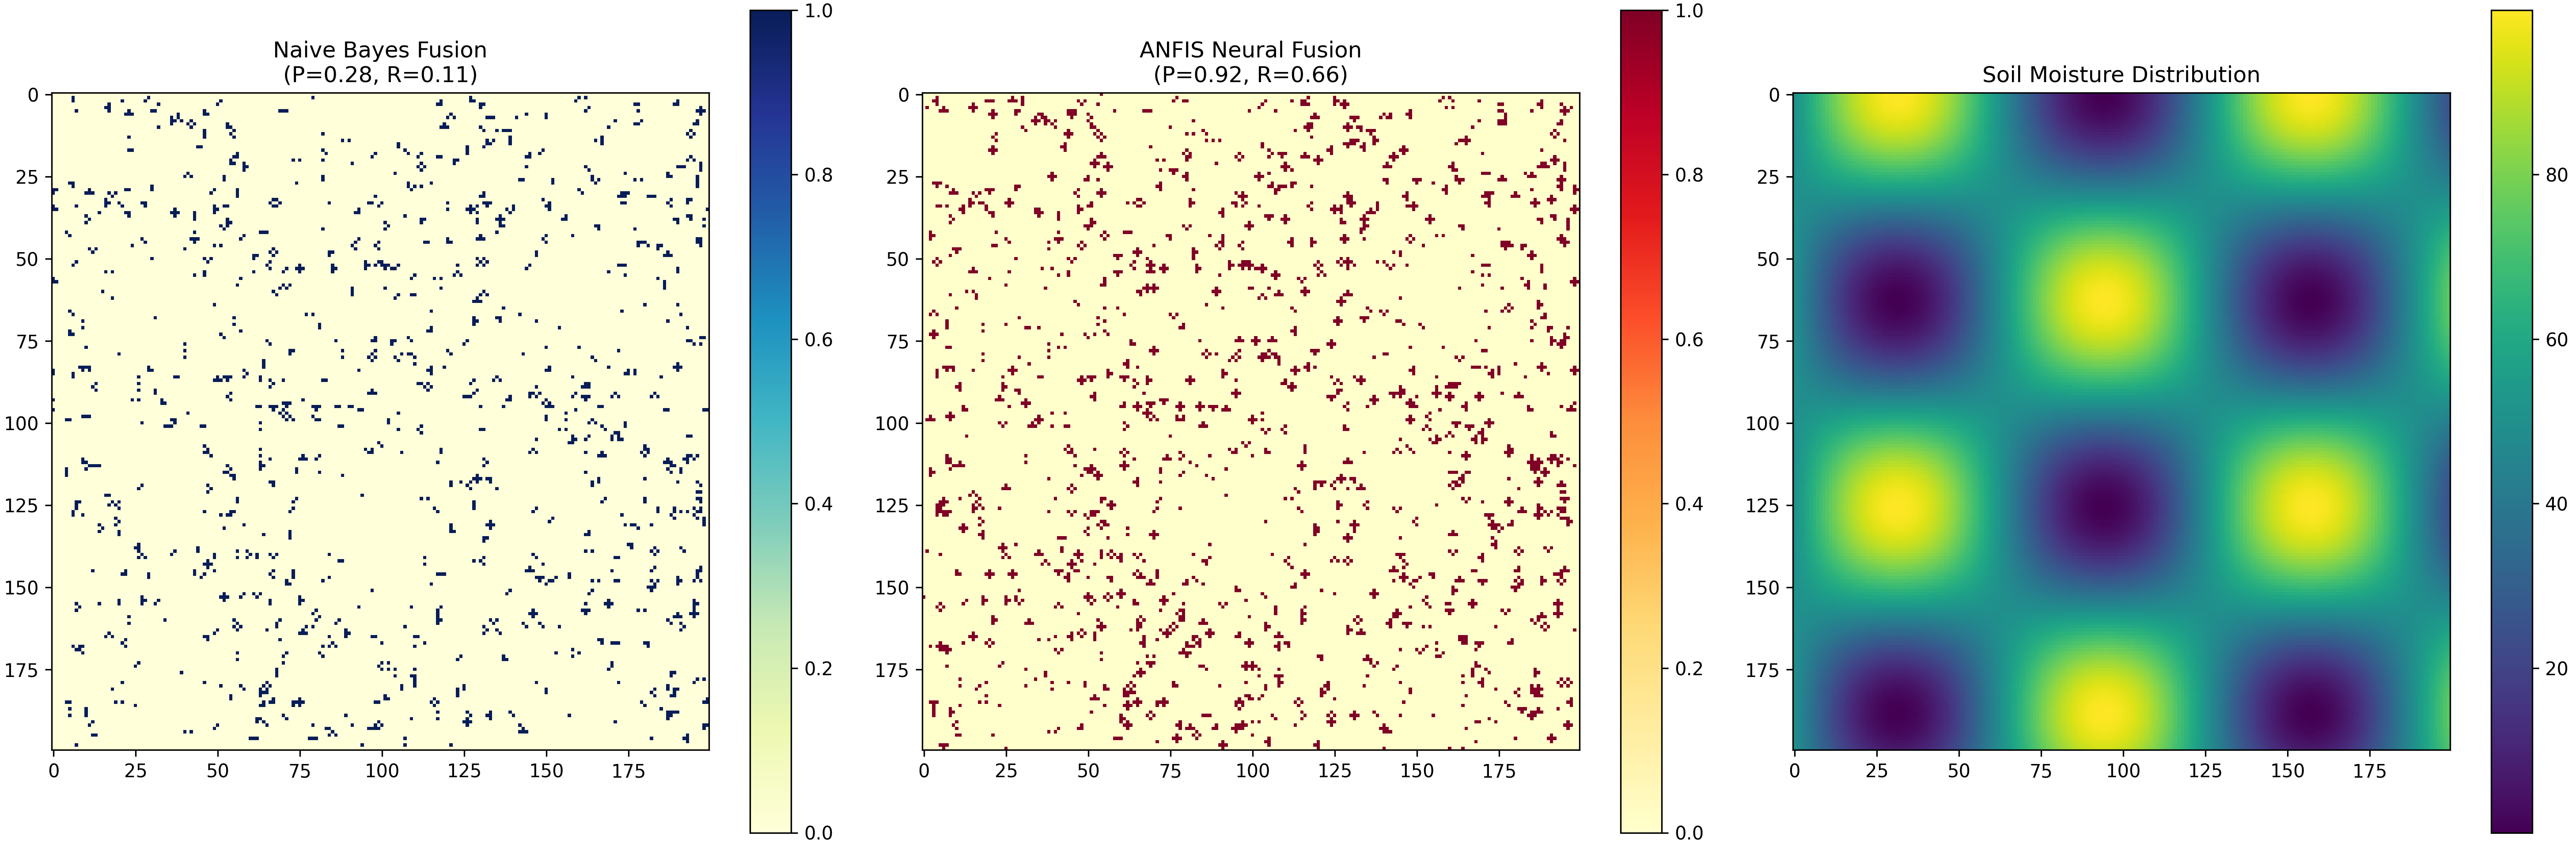
\includegraphics[width=0.98\textwidth]{figs/Rory/0_summary.png}
        \caption{ANFIS NB comparison summary. \textbf{Left:} simulated fusion for Naive Bayes. \textbf{Centre:} simulated fusion for ANFIS. \textbf{Right:} soil moisture distribution}
        \label{fig:anfis_summary}
    \end{figure}

    \paragraph{Future Work} 

        Several other physics-driven fusion algorithms exist. Another such approach is \textit{Physics Based Deep Learning} (PBDL)\footnote{\url{https://www.physicsbaseddeeplearning.org/intro.html}}, which benefits from implementing the physical domain knowledge at a deeper level in the \textit{model architecture and loss function}. PBDL is a recent field in Artificial Intelligence (AI), and it may have significant benefits, such as greater robustness to environmental variations in data-fusion for the detection of landmines.
